\section{Algorithms}

\subsection{B and B+ Algorithms}
% kenny, put a section here about B+ algorithms
The theory for the implementation was deceptively simple, since we had worked it out on paper in class, 
and the algorithms were simple enough to read through.  However general human intuition turned out to 
be fairly complicated to translate into usable Javascript code.  In order of complexity of implementation 
we had the general tree and node object structue, then the search methods, followed distantly by the insertion 
and deletion methods, which turned out to be quite complex to implement appropriately.

    Setting up the general structure for the objects that would represent our trees and the nodes that make them up 
was simple enough.  For B trees we created an object with properties to hold a master list of all nodes in the tree, 
the order of the tree, a direct reference to the tree's root node, a counter forthe number of nodes in the tree, and 
references to the methods for searching, insertion, and deletion methods, as well as a helper method called \texttt{insertUp}, 
which is called recursively after a node overflows to handle splitting the node and inserting the appropriate key into 
the parent node.  For B+ trees, the object we created has almost all the same properties, but its \texttt{insertUp} method is 
only for internal node overflow handling, and it also has a reference to a method called \texttt{bp\_leaf\_split} which handles 
overflow in a leaf node.

The node objects we created were designed to be used for both tree structures.  They contain a list of the values/keys 
in the node, a list of the children to the node, a reference to the node's parent, counters for the number of values/keys 
and for the number of children, a flag to signify if the node is a leaf node, and a reference to a helper method that returns 
the list of children to the node. The tree objects maintain a list of all the nodes in the tree because Javascript does not 
have easy to use pointers, so a master list had to be maintained so we could reference specific nodes as need be.  
As such, all references to nodes outside the master list, such as those inside nodes referencing children and its parent, are stored 
as the index of the node in the master list.  This method has the same memory footprint as a method that would have used pointers, 
though it adds a few extra lines of code where we have to constantly reference back to the trees node list and look up the index
 value of whatever node we want to reference.

    Implementing search for the two tree types was fairly straight forward and was accomplished in as few as 27 lines of code.  
For B trees, the method for searching consists of starting at the root, inspecting in the search value is in the node, if not 
then we decide which child node it would be in and then recursively call the search function starting from the child node the value 
should be in.  If we encounter a dead end and have not yet found our value, then we return that the value did not exist in the tree.
If we do find the value we return the index of the node it was found in and a true flag to indicate that the value was found.  The 
method for searching a B+ tree was similar except we do not check to see if the search value is in the current node until we've 
reached a leaf node.  Until we reach a leaf we just decide which child to explore next and recursively call the search function 
starting from that child.  Once we've reached a leaf node, if we find the value in the node, we return the node index amd a true flag.  If we reach a leaf node, and it does not contain our search value, then we return falseto indicate the value does not exist
 in the tree.
 
    Implementing insertion into the trees was where things became a bit complicated.  Specifically having to handle overflow and node splitting.  The insertion mothed for B trees starts out fairly simple, we do a search through the tree for the insertion value.  Regardless of whether the value is found or not, the search method should return us the node that the value should be inserted into.  We then do a brute force insert into the node, temporarily ignoring order, just to get the nodes values sorted.  Once we have the value inserted, we check if the node is now overflowing or not, if not we are done and end the function.  If we do encounter over flow then we quickly calculate the median value and partition the values into two separate sets around the median, but neither including the median value.  We then pass the two sets of values, the median value, the index of the median value, and the current node to out insertUp method to handle the spliting of the node.  The insertUp method recieves these values and that check to see if the current node is the root node or not.  If we are splitting the root node then the split is easy enough to accomplish.  We create two new nodes that will become the children to the root, and each inherit half the children of the previous root.  We want to keep the root of the tree at index 0 in the array of all nodes in the tree for convenience, which is why the new nodes created are the children to our new root, and not one of the children and the new root node.  We assign the appropriate values and children to the new nodes, and set them to look at the root node as their parent, we then assign the the new root the median value from the split node, and set its children to include the new children nodes we have created.
    
    If the node to be split was instead a leaf or internal node then the method of splitting is slightly different.  In this case we are only creating one new node to the tree, all the appropriate values and children, if any exist, are split between the original node we are splitting and the new node we are creating to take in half the values, and possible half the children.  We then recursively call the insertUp method to insert the median value into the split node's parent.  The function will recurse until either no node needs to be split, or we've split the root node.
    
    Insertion for B+ trees in almost identical, except it has to handle an extra specific case that B trees do not deal with.  Splitting internal nodes and the root node function identically, but B+ trees behave differently than B trees when splitting leaf nodes, and so an extra method to handle this case called bp\_leaf\_split is implemented.  When splitting a leaf node, it is similar to splitting an internal node, with slight changes.  When splitting a leaf node, we split the node down the middle, but do not separate out the median value to be inserted up into the parent node.  Instead, we select the smallest value from the right side of the split node and insert that as a key into the parent node, this being because all values are stored at the leaf level in B+ trees.  After splitting a leaf node we then call the B+ tree's insertUp method to handle insertion of the new key and potential splitting of the parent node.
    
    After some tweaking and discussion about our implementation for deletion in both B and B+ trees was changed from our original intended method in exchange for a more streamlined, though more costly method.  In investigating methods for implementing deletion from B and B+ trees we found there to be two popular methods of accomplishing this task.  The first is the most obvious, but also the more complex of the two to implement.  It consists of search for the value in the tree, removing it from where it lies, and then if the node should underflow, borrow from or merge with sibling nodes, and if need be change keys in parent nodes, which could then result in underflow propagating upward in the tree, which in turn would need to be handled.  The other method suggested passing through the tree and restructuring it such that no underflow would occur when the value is removed.  We had originally intended to implement the first method, but found that in development that the way we had things structured made it mush easier to implement the second method.  Our implementation of this method was fairly straight forward.  We search for the value to be deleted, if we find it and no underflow will occur, we remove it and are done.  If underflow does occur, then utilizing the tree's master list of values in the tree, we reconstruct the tree from these values, less the deleted value.  Our implementation run approximately in time O(n log n), but for small n the effect on performance in negligible.

\subsection{Graph Layout Algorithms}
The UI portion of this project requires a sizable amount of
algorithmic work. The most difficult factor is the development of a
node layout algorithm that prevents node overlap, while also giving an
ideal spacing between the nodes in the tree. This is especially
important as the size of the tree grows.

A popular method for solving this problem is the use of the
force-based algorithm. This algorithm works well for spreading nodes
out over 2 or 3 dimensional space. However, it does not take into
account the movement limitations that are imposed in a B+
tree. Namely, the nodes in a B+ tree can only move horizontally except
for in the case of a node split or join.

A secondary issue with the use of force-based algorithms is that they
have a running time of O$(n^3)$. This long running time is not ideal
for large trees. Our design helps mitigate the issues presented by
this running time. Namely, the size of the tree that can be visible to
the user is limited by the available screen real estate. This limits
the number of nodes down to a reasonable level, and thus keeps our
running time within reason.

Force based algorithms operate by modeling interaction between the
graph nodes using equations borrowed from physics. Each node is
treated as an electrically charged particle, repelling the other nodes
in the graph according to Coulomb's Law. Each edge on the graph is
treated as a spring, attracting the two connected nodes according to
Hooke's Law. The simulation randomizes initial node positions and then
simulates each time step in the model until equilibrium is reached. At
equilibrium, the nodes should be placed in such a way that overlap is
minimized.

%% what we did
Adapting this algorithm to work with our constraints proved to be an
interesting challenge. Of primary concern was the limitation that each
node should stay on its own level in the tree throughout the
simulation. This problem turned to be simple to solve. We modified the
initial force-based algorithm so that nodes could only apply force on
the X coordinate plane.

After implementing this system, it became clear that there were still
some serious issues to address. The nodes in the tree were becoming
far to spread apart. Furthermore, they were also off-center from their
expected locations. After some experimentation, it was determined that
the issue sprouted from an assumption the original algorithm made. The
original algorithm assumed that all nodes would repel each-other, as
would make sense in a 2-dimensional model. Unfortunately, the same
rule did not apply for 1-dimensional models. The solution to this
problem was to modify the code in such a way that the nodes in the
model would only repel against other nodes on that level of the tree.

The next issue encountered was that of node ordering. In the
standard force-based algorithm, all edge endpoints for a given node
have the same $(x,y)$ coordinates, and ordering does not matter. In
the case of B and B+ Trees, this is not true. Not only does each node
have multiple edge endpoints, but ordering also is extremely
important.

The endpoint problem was trivially solved by simply adjusting our
$(x,y)$ coordinates for the parent node. The issue of ordering proved
to be a bit more difficult. The solution we designed relies on the
algorithm used to build the tree. This algorithm inserts nodes one at
a time in a left to right order. With this in mind, our force-based
algorithm inserts all new nodes at the proper level, but to the far
right of the graph. This causes all of the nodes to shift to the left
as the model reaches equilibrium. Because the nodes should not cross
each other on the x-axis, they should maintain the same ordering throughout.
%% WIP

\subsection{Example of Tree Construction}

\begin{figure}[htp!]
\centering
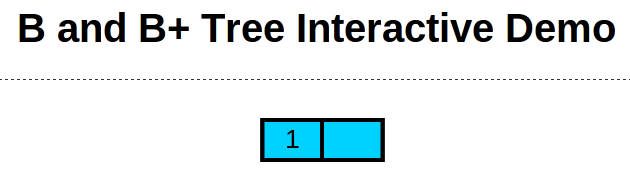
\includegraphics[scale=0.25]{images/Insert_one.png}
\caption{B tree after inserting value 1}
\label{EX1}
\end{figure}

\begin{figure}[htp!]
\centering

\includegraphics[scale=0.25]{images/Insert_two.png}
\caption{B tree after inserting value 2}
\label{EX2}
\end{figure}

\begin{figure}[htp!]
\centering
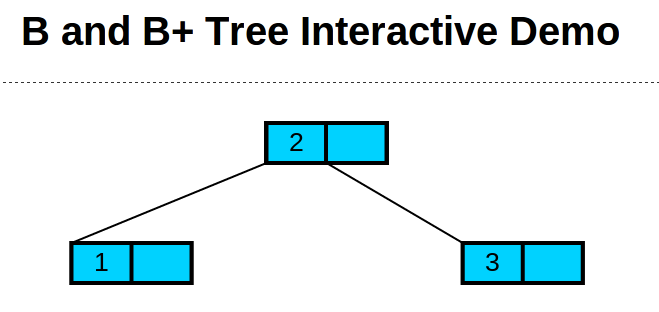
\includegraphics[scale=0.25]{images/Insert_three_split_root.png}
\caption{B tree after inserting value 3, splitting root}
\label{EX3}
\end{figure}

\begin{figure}[htp!]
\centering
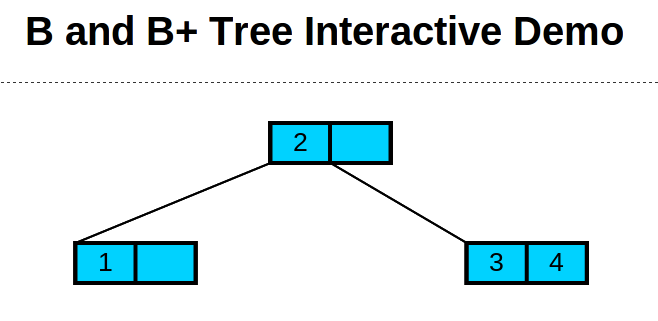
\includegraphics[scale=0.25]{images/Insert_four.png}
\caption{B tree after inserting value 4}
\label{EX4}
\end{figure}
\clearpage

\begin{figure}[htp!]
\centering
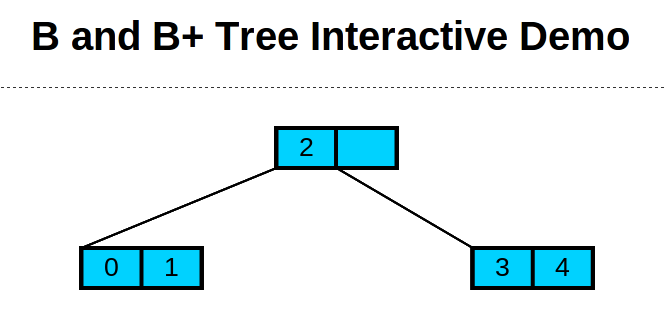
\includegraphics[scale=0.25]{images/Insert_zero.png}
\caption{B tree after inserting value 0}
\label{EX5}
\end{figure}
